\chapter{Risultati}\label{capitolo5risultati}
\vspace{4cm}

Riportiamo di seguito i tempi di runtime risultanti dall'esecuzione del programma su un pool di 100 dataset ottenuti grazie al generatore di cui al \autoref{capitolo4codice}. Per ogni dataset sono state eseguite 20 iterazioni in modo da evitare errori nell'analisi dovuti a momentanei picchi o crolli di prestazioni dell'hardware.

I kernel sono stati eseguiti sia su GPU che su CPU in modo da poter effettuare dei confronti, nello specifico:
\begin{itemize}
	\item{GPU: NVIDIA GeForce GTX 1650 with Max-Q Design}
	\item{CPU: Intel(R) Core(TM) i7-10710U @ 1.10GHz}
\end{itemize}

\begin{center}
\begin{scriptsize}
\bgroup
\def\arraystretch{1.5}
\begin{tabular}{|c|c|c|}
	\hline
	Device & \textbf{GPU} & \textbf{CPU} \\
	\hline
	Frequenza di clock & $\SI{1245}{\mega\hertz}$ & $\SI{1100}{\mega\hertz}$ \\
	\hline
	Core & 1024 & 6 \\
	\hline
	Migliore dimensione work-group & 32 & 128 \\
	\hline
	Host & Intel(R) Core(TM) i7-10710U & Intel(R) Core(TM) i7-10710U\\
	\hline
\end{tabular}
\egroup
\vspace{10pt}
\captionof{table}{Dettaglio sull'hardware usato per i test\label{tabellainfohw}}
\end{scriptsize}
\end{center}

%\begin{center}
%	\begin{scriptsize}
%\begin{figure}
%	\begin{tikzpicture}
%		\begin{axis}[
%			symbolic x coords={
%				$2^{13}$,
%				$2^{14}$,
%				$2^{15}$,
%				$2^{16}$,
%				$2^{17}$,
%				$2^{18}$,
%				$2^{19}$,
%			},
%			xtick=data,
%			width=\textwidth,
%			height=.5\textwidth,
%			x tick label style={rotate=45,anchor=east},
%			ylabel=Runtime ($\SI{}{\milli\second}$),
%			legend style={at={(1.1, 0.85)}, anchor=west},
%			ybar=0pt,
%			legend cell align={left},
%			enlarge x limits=0.1,
%			enlarge y limits=0.0,
%			]
%			\addplot+ coordinates { %CPU
%				($2^{13}$, 3.8242725)	
%				($2^{14}$, 6.962467143)
%				($2^{15}$, 10.79657)
%				($2^{16}$, 19.93930875)
%				($2^{17}$, 38.463008)
%				($2^{18}$, 80.91646625)
%				($2^{19}$, 180.4168033)
%			};
%			\addplot+ coordinates { %GPU
%				($2^{13}$, 5.274639225)
%				($2^{14}$, 6.876778213)
%				($2^{15}$, 7.679412375)
%				($2^{16}$, 8.08962315)
%				($2^{17}$, 11.881535)
%				($2^{18}$, 22.68048384)
%				($2^{19}$, 52.01390498)
%			};
%			\legend{CPU, GPU}
%		\end{axis}
%	\end{tikzpicture}
%	\caption{Runtime in relazione al numero di task del dataset}
%\end{figure}
%\end{scriptsize}
%\end{center}

%\centering 
\begin{center}
\begin{figure}
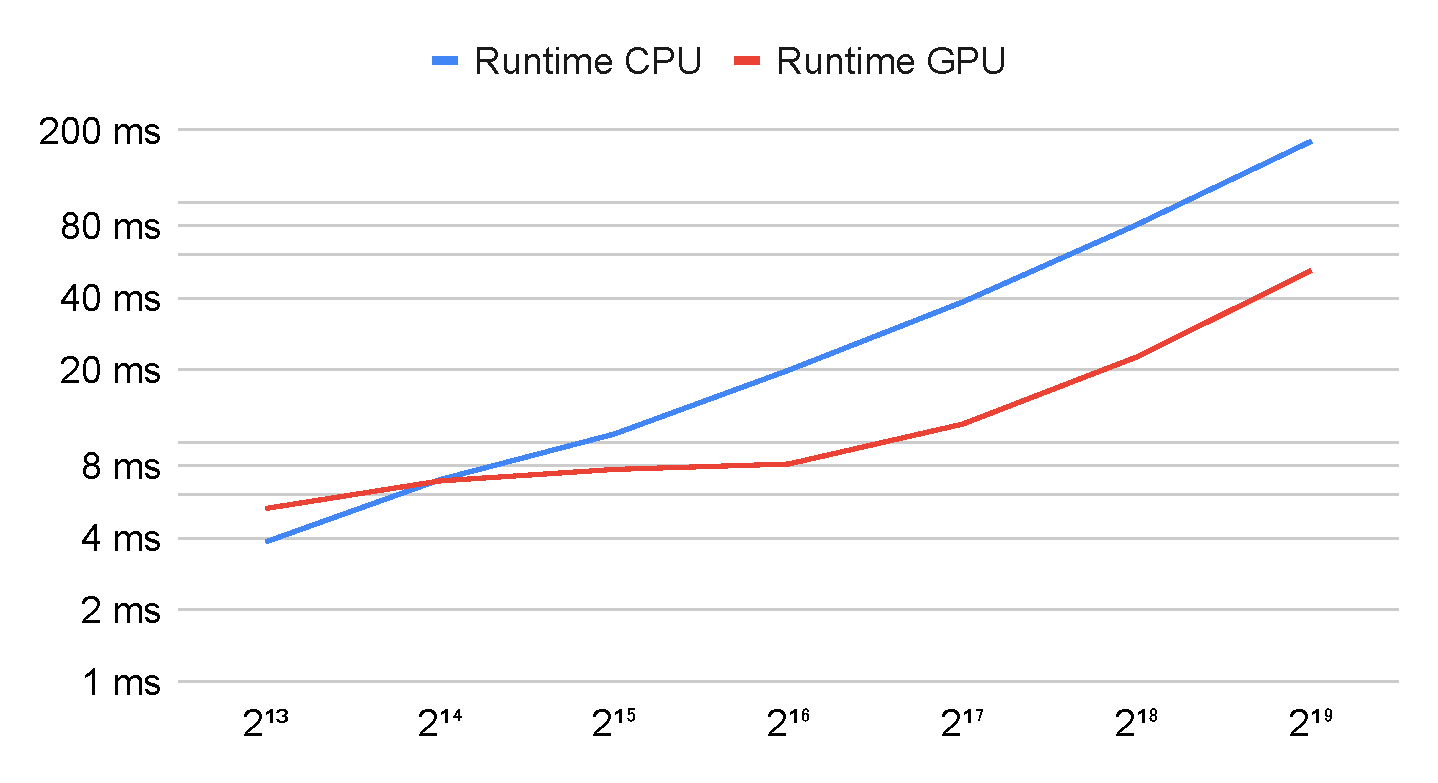
\includegraphics[width=\textwidth]{Images/runtime_total.pdf}
\caption{Tempi totali di runtime in relazione al numero di task del dataset. Grafico in scala logaritmica.}
\label{runtimetotal}
\end{figure}
\begin{figure}
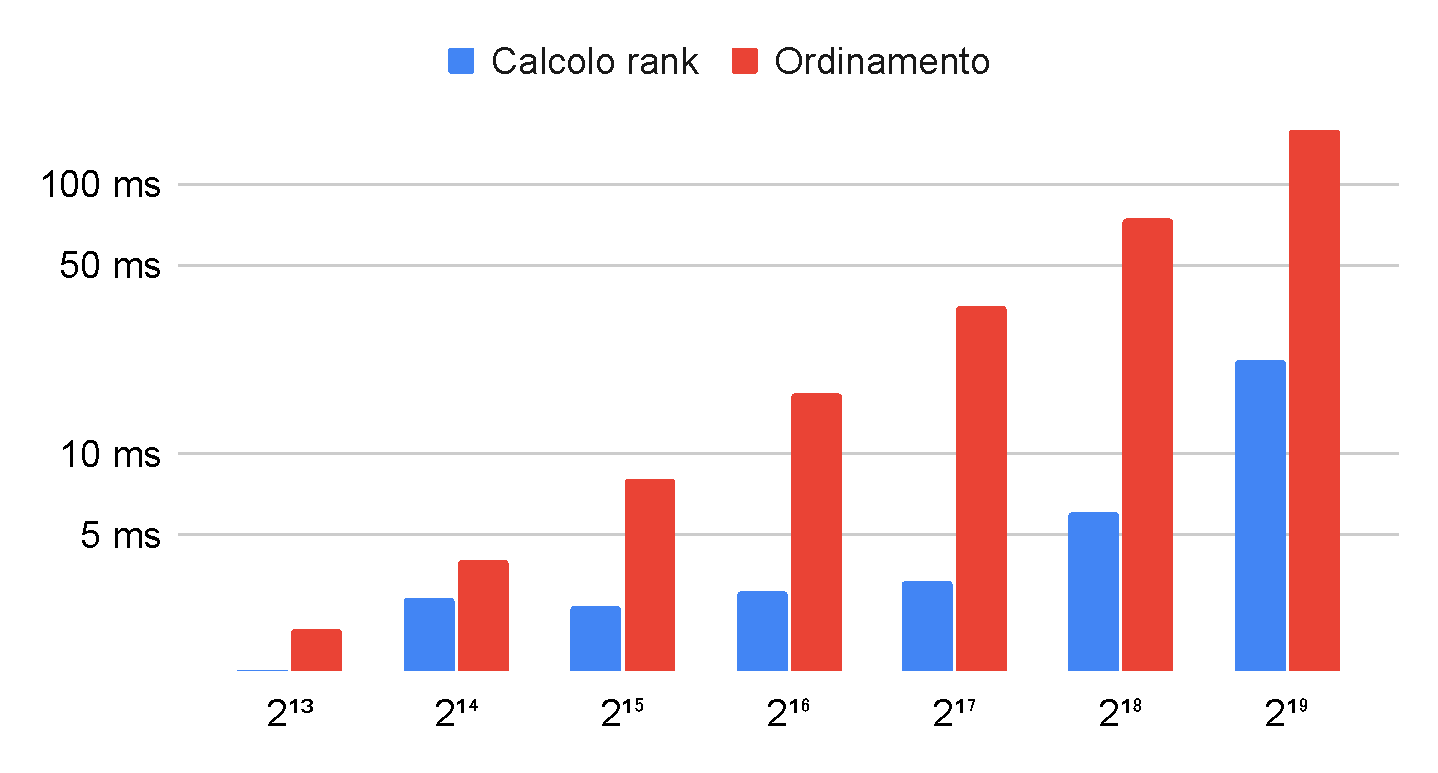
\includegraphics[width=\textwidth]{Images/kernel_cpu.pdf}
\caption{Dettaglio tempi di runtime per i kernel \textit{compute\_metrics} e \textit{bitonic\_mergesort} eseguiti su CPU, in relazione al numero di task del dataset. Grafico in scala logaritmica.}
\label{runtimegpu}
\end{figure}
\begin{figure}
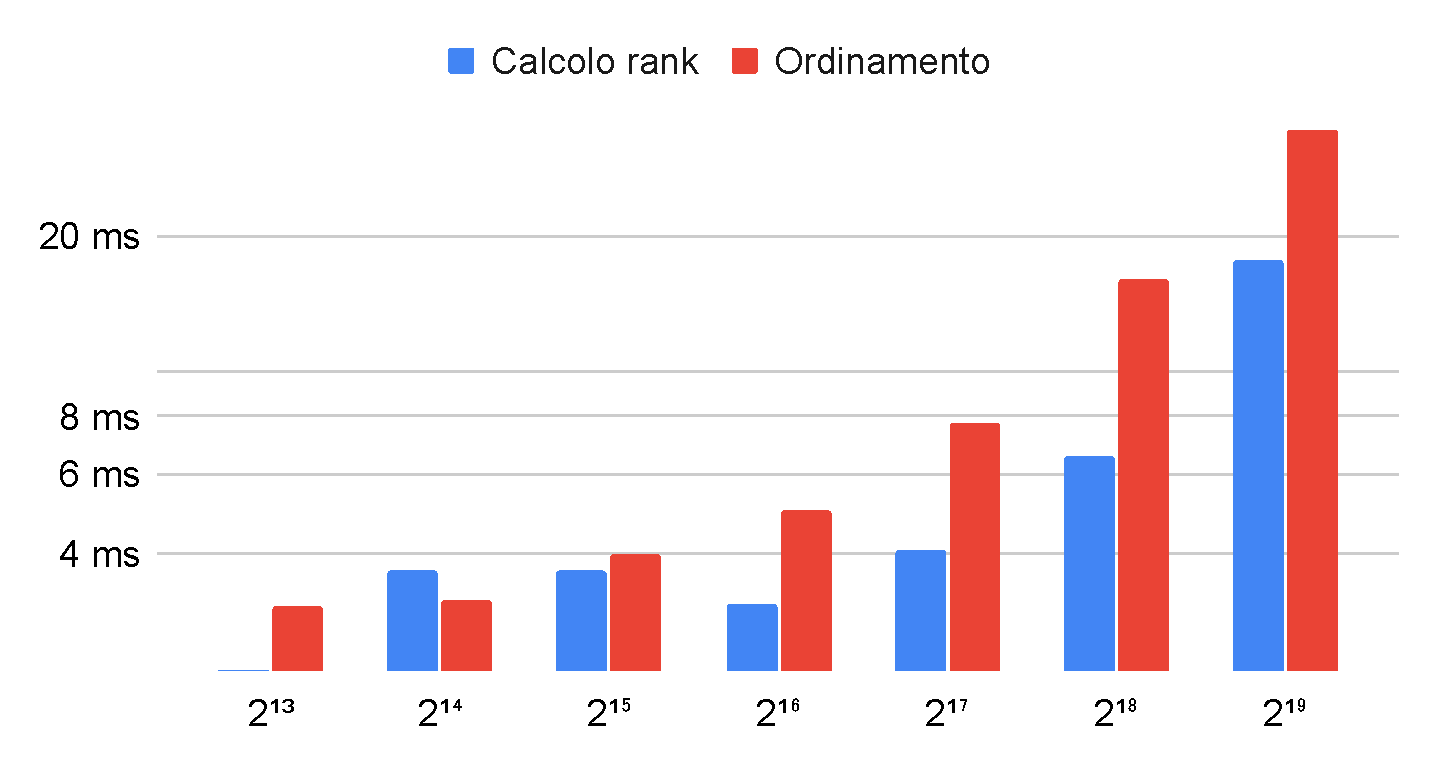
\includegraphics[width=\textwidth]{Images/kernel_gpu.pdf}
\caption{Dettaglio tempi di runtime per i kernel \textit{compute\_metrics} e \textit{bitonic\_mergesort} eseguiti su GPU, in relazione al numero di task del dataset. Grafico in scala logaritmica.}
\label{runtimecpu}
\end{figure}
\end{center}
\newpage
Si noti che, in questi grafici, non sono stati riportanti i tempi riguardanti la prima e l'ultima fase dell'algoritmo, questo perché il primo kernel ha tempi d'esecuzione trascurabili rispetto agli altri mentre l'ultimo viene eseguito serialmente dalla stessa macchina host, fornendo quindi gli stessi risultati in termini di tempi d'esecuzione.

\section{Confronto tra prestazioni attese e prestazioni effettive}
Tenendo conto dei dati teorici riguardanti la memory bandwidth delle varie piattaforme possiamo determinare se questo algoritmo riesce effettivamente a sfruttare al meglio tutti i device oppure se uno di questi performa meno di quanto dovrebbe.

In particolare le memorie dei device su cui sono stati eseguiti i test hanno banda passante teorica pari a:
\begin{itemize}
	\item GPU: $\SI{121.1}{\giga\byte/\second}$
	\item CPU: $\SI{15.0}{\giga\byte/\second}$ (Dovuta al bus PCIe 3.0)
\end{itemize}
da cui ne deriva una ratio pari a circa $8:1$ tra GPU e CPU.

I valori dei test ottenuti rivelano invece una ratio di circa $3.5:1$ per grandi dataset calcolata facendo una stima dei byte letti e scritti in media dai kernel e dividendo questa cifra per il tempo di runtime.

Ne deduciamo che la GPU non è effettivamente sfruttata a pieno e che probabilmente le cause di questa mancanza sono da ricercare nella frammentazione della coda dei task da analizzare nella fase 2 e nello scambio di informazioni con l'host necessario a terminare l'iterazione dei kernel di calcolo della metrica e di ordinamento finale.

Il primo di questi problemi è dovuto al fatto che la coda, nella sua implementazione attuale, contiene un valore non nullo nelle posizioni dell'array che corrispondono ai nodi da analizzare. Per ovviare a questo problema si potrebbe pensare di usare una coda effettiva invece di un array, tuttavia questo non è possibile perché i work-item dovrebbero sincronizzarsi per decidere a quale indirizzo poter inserire il nuovo nodo da aggiungere alla coda.

Anche il secondo problema non è risolvibile a causa dell'impossibilità di sincronizzare work-item di work-group diversi, per cui è necessario ritornare il controllo all'host in modo che possa verificare, attraverso una riduzione parallela, se è ancora necessario proseguire con un'altra esecuzione del kernel. 

\section{Andamento delle prestazioni}
Come si evince dalla \autoref{runtimetotal}, i tempi di runtime su GPU seguono un andamento lineare per piccoli dataset, questo perché il potenziale della GPU non viene sfruttato appieno e, di conseguenza, è più prestante la CPU.
Man mano che la grandezza dei dateset aumenta, si nota un'inversione di tendenza che vede i tempi su GPU consolidarsi al di sotto di quelli CPU, sebbene entrambi abbiano un andamento quadratico in linea con l'analisi di complessità riportata nella \autoref{analisicomputazionale}.

Per quanto riguarda i singoli kernel, notiamo come l'ordinamento richieda un tempo visibilmente più lungo degli altri kernel sia su GPU (per grandi dataset) che su CPU dove però il runtime cresce esponenzialmente al crescere del numero di task, mentre il kernel per il calcolo del rank risulta essere confrontabile tra i due device fino ai dataset contenenti $2^{18}$ task, a partire da questi, infatti, i risultati sono migliori sulla GPU.
